\subsection{Two-Body Density Matrix in Richardson Solution}
As pointed in \cite{Leggett}, the existing of eigenvalue in order of $N$ in the two-body density matrix of BCS solution is probably the most fundamental fact of the superfluid phenomenon.  In the traditional BCS ansatz, the order parameter $F_\vk=u_\vk v^*_\vk$ is this eigenvector with the eigenvalue of $N_0=\frac{\pi}4\Delta{}N(0)\Omega$, \cite[(5.4.32)]{Leggett}.  Therefore it is important to check the solution with Richardson approach \cite{CobosonBcsRich} about this quantity.  What we are looking for is only zero-central-momentum eigenfunction, 
\begin{equation}\label{eq:2bodyDensityMatrixDef}
\av{\beta_\vk^\dg\beta_{\vk'}^{}}=\av{a_\vk^\dg{}b_{-\vk}^\dg{}b_{-\vk'}^{}{}a_{\vk'}^{}}
\end{equation}
Here we mostly follow the original paper's notion, with some short-hand explained as following:
\begin{equation}
 B^\dg_i=B^\dg(R_i)
\end{equation}
\begin{equation}
 \avt{i}{\vk}=\avv{B_i^{}\beta^\dg_\vk}
\end{equation}
\begin{equation}
 \avt{i}{j}=\avv{B_i^{}B^\dg_j}=\sum_\vk \avt{i}{\vk} \avt{\vk}{j}
\end{equation}

In the Richardson solution, ground wave-function is $\ket{\Psi_n}=\prod_i^n{}B^\dg_i\ket{\nu}$. Here different $B^\dg_i\ket{\nu}$'s are neither orthogonal nor normalized. In fact, they have rather substantial overlap most of the time.   Two-body density matrix here is further complicated by the fact that many-body wave-function is affected by the \emph{composite} nature of those cobosons. Generally,  
\begin{equation}
\av{\beta_\vk^\dg\beta_{\vk'}^{}}=\frac{\avv[\Psi_n]{\beta_\vk^\dg\beta_{\vk'}^{}}}{\avt{\Psi_n}{\Psi_n}}
\end{equation}.   

\subsubsection{Two pairs}
We started with a two-pair state, $\ket{\Psi_2}=B^\dg_i{}B^\dg_j\ket{\nu}$. 

\begin{equation}\label{eq:tbdm2pair}
\begin{split}
 &\avv[\Psi_2]{\beta_\vk^\dg\beta_{\vk'}^{}}\\
=&\mbr{\br{\avt{i}{j}\avt{j}{\vk}\avt{\vk'}{j}+\avt{i}{j}\avt{j}{\vk}\avt{\vk'}{i}}+(i\leftrightarrow{}j)}\\
  &-2\mbr{\br{\avt{j}{\vk}\avt{i}{\vk}\avt{\vk}{i}\avt{\vk'}{j}+\avt{\vk'}{i}\avt{\vk'}{j}\avt{j}{\vk}\avt{i}{\vk'}}+(i\leftrightarrow{}j)}\\
&+4\avt{j}{\vk}\avt{i}{\vk}\avt{\vk'}{i}\avt{\vk'}{j}\delta_{\vk\vk'}
\end{split}
\end{equation}
Here the first four terms (fig. \ref{fig:tbdm2pair1},\ref{fig:tbdm2pair2}) are from the paring, while the next eight terms (fig. \ref{fig:tbdm2pair3}-\ref{fig:tbdm2pair6}) as well as the last term  (fig. \ref{fig:tbdm2pair7}) are due to the Pauli exclusion of \emph{composite} nature. They show the moth-eaten effect.
\begin{figure}[htb]
\centering
  \subfloat[][]{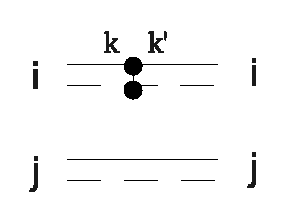
\includegraphics[width=0.2\textwidth]{image/tbdm2pair1.eps}\label{fig:tbdm2pair1}}\qquad
 \subfloat[][]{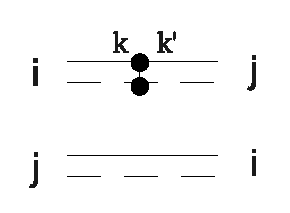
\includegraphics[width=0.2\textwidth]{image/tbdm2pair2.eps}\label{fig:tbdm2pair2}}\qquad
  \subfloat[][]{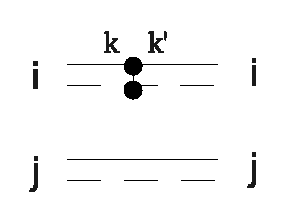
\includegraphics[width=0.2\textwidth]{image/tbdm2pair1.eps}\label{fig:tbdm2pair3}}\\
 \subfloat[][]{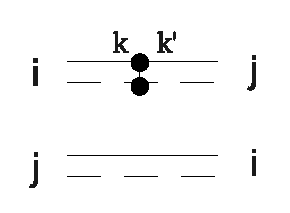
\includegraphics[width=0.2\textwidth]{image/tbdm2pair2.eps}\label{fig:tbdm2pair4}}\qquad
  \subfloat[][]{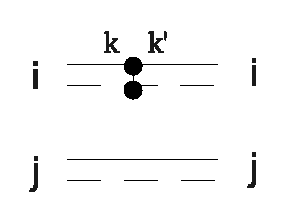
\includegraphics[width=0.2\textwidth]{image/tbdm2pair1.eps}\label{fig:tbdm2pair5}}\qquad
 \subfloat[][]{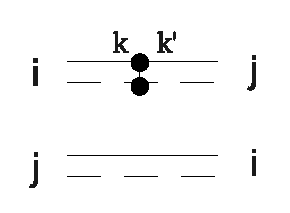
\includegraphics[width=0.2\textwidth]{image/tbdm2pair2.eps}\label{fig:tbdm2pair6}}\\
  \subfloat[][]{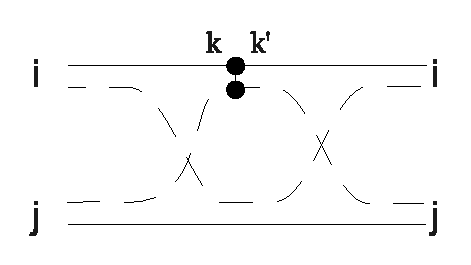
\includegraphics[width=0.3\textwidth]{image/tbdm2pair7.eps}\label{fig:tbdm2pair7}} 
\caption{Shiva diagram of two pairs }
\begin{description}
\item[\subref{fig:tbdm2pair1},\subref{fig:tbdm2pair2}] Signle pair without Pauli scattering.  There are also terms with $(i\leftrightarrow{j})$. First line of the above equation. 
\item[\subref{fig:tbdm2pair3},\subref{fig:tbdm2pair4},\subref{fig:tbdm2pair5},\subref{fig:tbdm2pair6}] Two-pair with Pauli scattering.  There are also terms with $(i\leftrightarrow{j})$. 
Second line of the equation. 
\item[\subref{fig:tbdm2pair7}] This coresponds the last term.  And there are the permutation of (i,j) as other terms.  
\end{description}
\end{figure}

The last term is especially interseting as this is two separate pieceses (fig.\ref{fig:shivaseparate}).  Normally, they do not exist, but here they do show up because we need pair of $\vk$,$\vk'$ .  
\begin{figure}[htb]\centering
 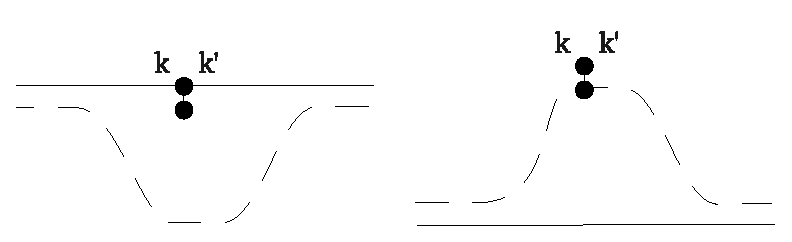
\includegraphics[width=0.3\textwidth]{image/shivaSeparate.eps}
\caption{Two separate connection parts of the last term of \eqref{eq:tbdm2pair}\label{fig:shivaseparate}}\centering
\end{figure}
And the normalization factor:
\begin{equation}
 {\avt{\Psi_2}{\Psi_2}}=\av{B^{}_j{}B^{}_i{}B^\dg_i{}B^\dg_j}=\avt{i}{i}\avt{j}{j}+\abs{\avt{i}{j}}^2-2\sum_\vk\avt{j}{\vk}\avt{i}{\vk}\avt{\vk}{i}\avt{\vk}{j}
\end{equation}

\subsubsection{Three pairs}
For a three-pair state $\ket{\Psi_3}=B^\dg_i{}B^\dg_j{}B^\dg_m\ket{\nu}$. 
we have 
\begin{equation}
\begin{split}
 \bra{\Psi_3}\beta^\dg_\vk=&\bra{\nu}B_m{}B_j{}B_i\beta^\dg_\vk\\
=&-2\avt{j}{\vk}\avt{m}{\vk}\bra{\nu}\beta_\vk{}B_i-2\avt{m}{\vk}\avt{i}{\vk}\bra{\nu}\beta_\vk{}B_j
-2\avt{i}{\vk}\avt{j}{\vk}\bra{\nu}\beta_\vk{}B_m\\
&+\avt{m}{\vk}\bra{\nu}B_i{}B_j+\avt{i}{\vk}\bra{\nu}B_j{}B_m+\avt{i}{\vk}\bra{\nu}B_m{}B_i\\
=&\br{-2\avt{i}{\vk}\avt{j}{\vk}\bra{\nu}\beta_\vk{}B_m+\avt{i}{\vk}\bra{\nu}B_j{}B_m}+(\mbox{i,j,m rotate permutation})
\end{split}
\end{equation}
We are lots of terms in the final expectation, like $\av{B^\dg{}B^\dg{}B^{}B^{}}$, $\av{\beta^\dg{}B^\dg{}B^{}B^{}}$,$\av{\beta^\dg{}B^\dg{}B^{}\beta^{}}$ , $\av{B^\dg{}B^\dg{}B^{}\beta^{}}$ .  